% Preamble del documento

\documentclass[11pt, a4paper, titlepage]{article}


%%%%%%%%%%%%%%%%%%%%%%%%%%%%%%%%%%%%%%%%%%%%%%%%%%%%%%%%%%%%%%%%%%%%%%%%%%%%%%%%%%%%%%%%%%%%%%%%
% Encoding e idioma Español, 
%%%%%%%%%%%%%%%%%%%%%%%%%%%%%%%%%%%%%%%%%%%%%%%%%%%%%%%%%%%%%%%%%%%%%%%%%%%%%%%%%%%%%%%%%%%%%%%%
\usepackage[utf8]{inputenc}
\usepackage[spanish, es-tabla]{babel} % Para poner cuadro en vez de tabla, etc
%%%%%%%%%%%%%%%%%%%%%%%%%%%%%%%%%%%%%%%%%%%%%%%%%%%%%%%%%%%%%%%%%%%%%%%%%%%%%%%%%%%%%%%%%%%%%%%%



%%%%%%%%%%%%%%%%%%%%%%%%%%%%%%%%%%%%%%%%%%%%%%%%%%%%%%%%%%%%%%%%%%%%%%%%%%%%%%%%%%%%%%%%%%%%%%%%
% Paquetes 
%%%%%%%%%%%%%%%%%%%%%%%%%%%%%%%%%%%%%%%%%%%%%%%%%%%%%%%%%%%%%%%%%%%%%%%%%%%%%%%%%%%%%%%%%%%%%%%%
\usepackage[colorlinks=true, urlcolor=cyan, citecolor=blue, linkcolor=blue, hidelinks]{hyperref} % /url{}, /ref{}...
\usepackage[a4paper,top=2cm,bottom=2cm,left=3cm,right=3cm,marginparwidth=1.75cm]{geometry}
\usepackage{minted} % Código
\usepackage{setspace}
\usepackage{pdfpages}

\usepackage[sorting=none, style=numeric]{biblatex} % aparece 1ro la 1ra citada
\addbibresource{citas.bib}

\usepackage{amsmath}

\usepackage[utf8]{inputenc} 

\usepackage[table]{xcolor} % Colores en tablas/texto/etc

\usepackage{graphicx} % Imágenes

\usepackage{tabularx} % Tablas más potentes
\usepackage{longtable} % Tablas muy largas
\usepackage{multirow}
\usepackage{booktabs}
\usepackage{multicol}
\usepackage{adjustbox} % Ajustar tablas al ancho de la página
\usepackage{pdflscape}

\usepackage{datetime} % Fechas
\usepackage{svg} % para el svg del logo de la eina
\usepackage{titlesec}
\usepackage[section]{placeins}  % para floatbarrier en secciones, 
                                % con [section] se ponen silenciosamente en cada seccion

\usepackage{listliketab}                                
\usepackage{fancyhdr} %pagestyles adicionales

\usepackage{lmodern} % Fuente moderna, \code con negrita
\usepackage{caption} % para poner labels en tabular sin convertirlos en tablas que flotan

\makeatletter
%%%%%%%%%%%%%%%%%%%%%%%%%%%%%%%%%%%%%%%%%%%%%%%%%%%%%%%%%%%%%%%%%%%%%%%%%%%%%%%%%%%%%%%%%%%%%%%%
\renewcommand\paragraph{\@startsection{paragraph}{4}{\z@}%
            {-2.5ex\@plus -1ex \@minus -.25ex}%
            {1.25ex \@plus .25ex}%
            {\normalfont\normalsize\bfseries}} % no sé de donde ha salido esto
\makeatother
\setcounter{secnumdepth}{4} % how many sectioning levels to assign numbers to
\setcounter{tocdepth}{4}    % how many sectioning levels to show in ToC
%\setlength{\parindent}{0pt} % para quitar indentación inicial en párrafos

%%%%%%%%%%%%%%%%%%%%%%%%%%%%%%%%%%%%%%%%%%%%%%%%%%%%%%%%%%%%%%%%%%%%%%%%%%%%%%%%%%%%%%%%%%%%%%%%
% Título para \maketitle
%%%%%%%%%%%%%%%%%%%%%%%%%%%%%%%%%%%%%%%%%%%%%%%%%%%%%%%%%%%%%%%%%%%%%%%%%%%%%%%%%%%%%%%%%%%%%%%%
\title{Plantilla de trabajo}
\author{autor1 \and autor2 \and autor3}

% Macro para mostrar el mes y el año (https://texnique.fr/osqa/questions/1359/commandes-month-year)
\def\monthyear{\ifcase\month\or
  Enero\or Febrero\or Marzo\or Abril\or Mayo\or Junio\or
  Julio\or Agosto\or Septiembre\or Octubre\or Noviembre\or Diciembre\fi
  \space\number\year}

\date{\monthyear}
%%%%%%%%%%%%%%%%%%%%%%%%%%%%%%%%%%%%%%%%%%%%%%%%%%%%%%%%%%%%%%%%%%%%%%%%%%%%%%%%%%%%%%%%%%%%%%%%


%%%%%%%%%%%%%%%%%%%%%%%%%%%%%%%%%%%%%%%%%%%%%%%%%%%%%%%%%%%%%%%%%%%%%%%%%%%%%%%%%%%%%%%%%%%%%%%%
% Estilos
%%%%%%%%%%%%%%%%%%%%%%%%%%%%%%%%%%%%%%%%%%%%%%%%%%%%%%%%%%%%%%%%%%%%%%%%%%%%%%%%%%%%%%%%%%%%%%%%
%\pagestyle{fancy} % con el nombre de la sección y página arriba
%\fancyhf{}
%\pagenumbering{arabic}
%\rfoot{Page \thepage}
\newcommand{\code}{\texttt} % para poner codigo en Monospace


\pagestyle{fancy}
\fancyhf{}
%\rhead{\rightmark}
\lhead{\leftmark}
\rfoot{\thepage}
%%%%%%%%%%%%%%%%%%%%%%%%%%%%%%%%%%%%%%%%%%%%%%%%%%%%%%%%%%%%%%%%%%%%%%%%%%%%%%%%%%%%%%%%%%%%%%%%

% Fin del preamble

% Forza las opciones desde el principio del documento si no se aplican
\AtBeginDocument{
  \urlstyle{same}
  \addtocontents{toc}{\small}
  \addtocontents{lof}{\small}
}
% Cuerpo del documento
\begin{document} 


%%%%%%%%%%%%%%%%%%%%%%%%%%%%%%%%%%%%%%%%%%%%%%%%%%%%%%%%%%%%%%%%%%%%%%%%%%%%%%%%%%%%%%%%%%%%%%%%%		
% PORTADA
%%%%%%%%%%%%%%%%%%%%%%%%%%%%%%%%%%%%%%%%%%%%%%%%%%%%%%%%%%%%%%%%%%%%%%%%%%%%%%%%%%%%%%%%%%%%%%%%
\begin{titlepage}

\thispagestyle{empty}
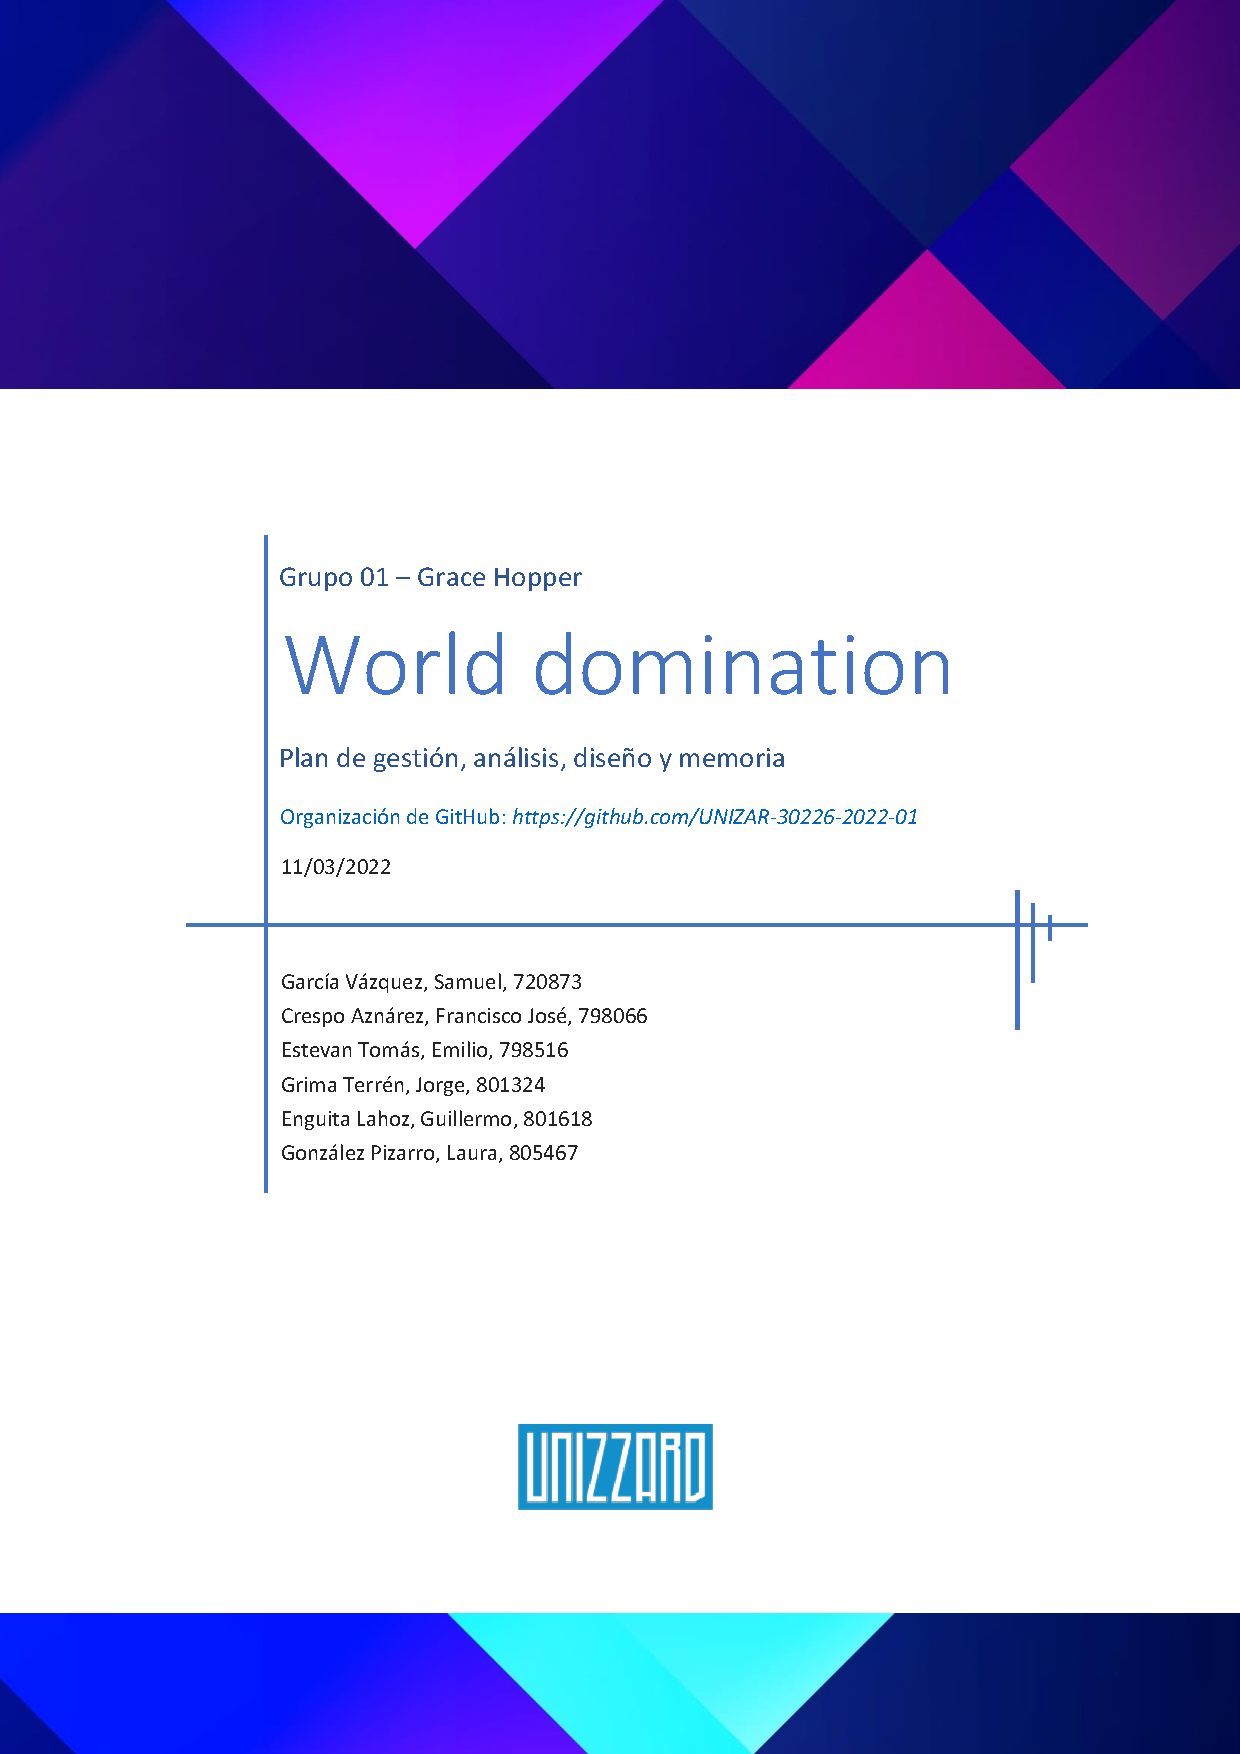
\includepdf[]{portadaMemoria.pdf}

\end{titlepage}
\newpage
%%%%%%%%%%%%%%%%%%%%%%%%%%%%%%%%%%%%%%%%%%%%%%%%%%%%%%%%%%%%%%%%%%%%%%%%%%%%%%%%%%%%%%%%%%%%%%%%





%%%%%%%%%%%%%%%%%%%%%%%%%%%%%%%%%%%%%%%%%%%%%%%%%%%%%%%%%%%%%%%%%%%%%%%%%%%%%%%%%%%%%%%%%%%%%%%%%		
% CUERPO
%%%%%%%%%%%%%%%%%%%%%%%%%%%%%%%%%%%%%%%%%%%%%%%%%%%%%%%%%%%%%%%%%%%%%%%%%%%%%%%%%%%%%%%%%%%%%%%%
\thispagestyle{empty}
\fontsize{11pt}{11pt}\selectfont

\setcounter{tocdepth}{4}

% Índice con links en negro y no en azul
{
    \hypersetup{linkcolor=black}
    \doublespacing
    \tableofcontents
}

\thispagestyle{empty}

% Texto
\clearpage
\setcounter{page}{1}
\section{Introducción}
A lo largo del documento se va a presentar un proyecto que se ha denominado\textit{ \textbf{World Domination}}. Se trata de un juego de estrategia \textit{on-line} por turnos e inspirado en \textit{Risk}, en el que cada jugador lucha contra el resto por la dominación del mundo. Cada uno de los jugadores cuenta con un número de soldados y territorios controlados por los mismos, así como con una baraja de cartas propia que serán canjeadas por más soldados. En cada turno, los jugadores tendrán que luchar contra tropas bajo el dominio de los rivales, decidiéndose los resultados mediante tiradas de dados. \newline

El juego proporcionará funcionalidades adicionales, que permitirán disfrutar de una experiencia social, fomentando la competición y una mayor participación en futuras partidas. \newline

El sistema debe ser capaz de gestionar las cuentas de los usuarios junto con las partidas que se desarrollen, así como la gestión de turnos y la inicialización y finalización de cada una de las partidas. Algunos de los objetivos fundamentales del sistema son: 

\begin{itemize}
\item Se permitirá a los usuarios registrarse e iniciar sesión con sus credenciales, que constan de un \textit{email} y contraseña. El uso de una cuenta de usuario será necesario para jugar partidas.

\item El sistema contará con una clasificación global de los mejores jugadores y de sus respectivas puntuaciones de las partidas jugadas.

\item Se permitirá a los usuarios personalizar elementos del juego en función de sus preferencias, como las fichas, su foto de perfil, o los dados usados durante las partidas.

\item El sistema recompensará al usuario por haber jugado o ganado un número determinado de partidas con puntos canjeables en la tienda del juego. La tienda será el punto de compra de personalizaciones de los elementos del juego.

\item Se permitirá gestionar una lista de amigos de cada usuario.

\item El sistema permitirá crear partidas públicas y privadas, conforme a las siguientes reglas:
\begin{itemize}
    \item Las partidas serán de 2 a 6 jugadores.
    \item Se permitirá a cualquier usuario entrar a partidas públicas.
    \item En el caso de partidas privadas, solo se permitirá la entrada con una contraseña, introducida al crearla.
    \item Se encontrará disponible un \textit{chat} en la partida.
    \item Se restringirá al usuario a poder jugar solo una partida al mismo tiempo.
\end{itemize}

\item Las partidas se desarrollarán de forma asíncrona, permitiendo a los usuarios responder en cualquier momento. Si el usuario se encuentra conectado, podrá ver una notificación en la pantalla. En el caso contrario, se enviará un correo al mismo notificando que puede realizar la jugada.

\item Habrá un mecanismo de expulsión de jugadores que no respondan o realicen jugadas en un tiempo determinado.

\end{itemize}

A lo largo de la realización del proyecto, será necesario realizar algunas entregas del trabajo llevado a cabo, en reuniones propuestas en unos plazos establecidos:

\begin{itemize}
    \item Una reunión para la evaluación de todas las funcionalidades del juego, con el sistema implementado en una versión final, con el objetivo de realizar ajustes finales, en la semana del 16 al 20 de Mayo.
    \item El sistema final se entregará no más tarde del 1 de junio, con los cambios propuestos durante las reuniones intermedias.
\end{itemize}

A continuación se hablará sobre otros aspectos del proyecto, de la gestión, la organización, análisis de requisitos, así como del diseño del sistema.

\section{Organización del proyecto}
El equipo está formado por 6 integrantes: Samuel García, Guillermo Enguita, Laura Gonzalez, Francisco Crespo, Emilio Estevan y Jorge Grima.
Hemos dividido el proyecto en tres bloques fundamentales:\newline
\begin{itemize}
    \item \textit{Backend} implementado con \textbf{Go} y desarrollo de la API.
    \item Primera versión del \textit{frontend} implementada con \textbf{React}.
    \item Segunda versión del \textit{frontend} implementada con \textbf{Angular}.\newline
\end{itemize}

El trabajo del primer bloque será llevado a cabo por Samuel y Guillermo, el del segundo bloque por Francisco y Emilio, mientras que el del tercer bloque será realizado por Laura y Jorge. 
Aunque cada uno tenga un bloque asignado, en todo momento se ayudará a integrantes encargados del trabajo en otros bloques si fuera necesario. \newline

El equipo decidió nombrar como director a Francisco Crespo, encargado de llevar a cabo la organización principal del proyecto, así como de las entregas necesarias del trabajo.

\section{Plan de gestión del proyecto}

A continuación, se describe cómo se llevaran a cabo distintas tareas a realizar en diferentes momentos del proyecto, como pueden ser: plan inicial de trabajo, división del trabajo a realizar o control de creación de software, entre otros.

\subsection{Inicio del proyecto}

\begin{itemize}

\item En primer lugar, en referencia a formación común del equipo y, debido a que la completitud de la documentación necesaria para el proyecto va a ser realizada en \textbf{Latex}, todos los miembros del equipo han adquirido conocimientos básicos para la utilización y explotación de esta herramienta. Para lograr este objetivo, se han realizado dos tutoriales. El primero de ellos <<Learn LaTeX in 30 minutes>>\cite{latextutorial1}se puede encontrar en la página web de \textit{Overleaf}. A su vez, se han seguido los manuales de ayuda proporcionados por la página oficial de \textit{Latex}\cite{latextutorial2}. 

\item Por otro lado, continuando en lo que respecta a la formación común, los integrantes del Grupo 1 asistieron a la práctica: \textit{Puesta en marcha de GitHub y fundamentos de Git} impartida por los profesores de la asignatura \textit{Proyecto Software}, la cual consistió en familiarizarse con la herramienta \textbf{Git} y su uso en conjunto con \textbf{GitHub}. A su vez, por medio del tutorial: \textit{Git, GitHub y Publicación Web}\cite{githubtutorial} se habían adquirido los conocimientos básicos de la respectiva tecnología.

\item Los encargados del desarrollo del \textit{backend} harán uso de \textbf{Go} como lenguaje de programación. Se trata de un lenguaje bastante conocido debido a que fue utilizado durante las prácticas de la asignatura \textit{Sistemas Distribuidos}. De cara a fijar conocimientos y a aprender nuevas mecánicas, fue realizado el tutorial de la página web oficial de \textbf{Go}. \\
Por otro lado, también realizaron una formación relacionada con las distintas \textit{APIs web}, concretamente el tutorial \textit{Introducción a las APIs web} de MozillaDeveloper\cite{apisweb}.

\item El equipo encargado del primer \textit{frontend}, implementado con \textbf{React}, necesita adquirir los conocimientos necesarios para trabajar con esta tecnología. Para ello, se realizará el tutorial oficial de \textbf{ReactJs}: \textit{Tutorial: Introducción a React}\cite{reactjs}, el cual consta de una duración estimada de 8 horas. A su vez, será realizado el tutorial de APIs web anteriormente mencionado\cite{apisweb}.

\item Por último, el equipo encargado de desarrollar el segundo \textit{frontend}, implementado con \textbf{Angular}. Debido a que no se ha trabajado con este \textit{framework} es necesario realizar un tutorial para aprender a usar esta tecnología. De cara a lograr este objetivo, será realizado el tutorial \textit{Angular y TypeScript}\cite{angular} proporcionado por \textit{DesarrolloWeb}, el cual tiene un tiempo estimado de realización próximo a las 7 horas.

\end{itemize}

\subsection{Control de configuraciones, construcción del software y aseguramiento de la calidad del producto}

Se han establecido los siguientes procedimientos relativos a las tareas de construcción del \textit{software}, gestión de incidencias, automatización, calidad y despliegue del sistema por completo.

\subsubsection{Convenciones y procedimientos para la construcción y control del software}

\begin{itemize}
    \item La organización y nombrado de los ficheros fuente seguirá las prácticas recomendadas por cada uno de los \textit{frameworks} a utilizar. De este modo, se seguirán las siguientes guías de estilo, nombrado de ficheros y organización de proyectos:
    \begin{itemize}
        \item Para \textbf{Angular}, se utilizará la guía de estilo oficial\cite{estiloangular} y la guía de estructura de proyectos propuesta por la documentación oficial\cite{estructuraangular}.
        
        \item Para \textbf{React}, se utilizará la
        guía de estilo de \textit{airbnb}\cite{estiloreact} y la estructura de proyectos propuesta por la documentación oficial\cite{estructurareact}.
        
        \item Para \textbf{Go}, se utilizará el estilo impuesto por la herramienta automática de formato de dicho lenguaje\cite{estilogolang} y la estructura de proyectos recomendada por la comunidad\cite{estructuragolang}, compatible con las herramientas de compilación del lenguaje.
    \end{itemize}
    
    \item Los ficheros de documentación no interna serán nombrados con minúsculas y podrán contener guiones bajos, sin caracteres especiales. Si forman parte de la documentación del código o interfaces, su nombre empezará por \textbf{documentacion\_}, y si forman parte de guías de uso para los clientes, su nombre empezará por \textbf{guia\_}.
    
    \item Todo el código será subido a los repositorios de la organización de \textbf{Github}\footnote{\href{https://github.com/UNIZAR-30226-2022-01}{\color{blue}{Repositorio de la organización de \textbf{Github}}}}, donde todos los miembros tendrán permisos de acceso, modificación y administración de los mismos. Los repositorios serán los siguientes:
    \begin{itemize}
        \item Un repositorio para el \textit{backend} del sistema\footnote{\href{https://github.com/UNIZAR-30226-2022-01/proyecto_software_backend}{\color{blue}{Repositorio del \textit{backend} del sistema}}}, en el cual se localizará todo el código y ficheros para el despliegue relativo al servidor de \textit{API} escrito en \textbf{Go}.
        
        \item Un repositorio para el \textit{frontend} de \textbf{React}\footnote{\href{https://github.com/UNIZAR-30226-2022-01/proyecto_software_frontend_react}{\color{blue}{Repositorio del frontend de \textbf{React}}}}, en el cual se localizará todo el código y ficheros para el despliegue relativo al frontend de \textbf{React}.
        
        \item Un repositorio para el \textit{frontend} de \textbf{Angular}\footnote{\href{https://github.com/UNIZAR-30226-2022-01/proyecto_software_frontend_angular}{\color{blue}{Repositorio del frontend de Angular}}}, en el cual se localizará todo el código y ficheros para el despliegue relativo al frontend de \textbf{Angular}.
        
        \item Un repositorio para la documentación pública\footnote{\href{https://github.com/UNIZAR-30226-2022-01/proyecto_software_documentacion}{\color{blue}{Repositorio de documentación pública}}}, en el cual se localizarán todos los archivos de documentación interna o para los clientes finales y parciales, como archivos de \LaTeX.
    \end{itemize}
    
    \item La gestión de incidencias y tareas pendientes se realizará mediante el gestor de incidencias de \textbf{GitHub} del repositorio relacionado con ellas.
    
    \item Todas las tareas, funcionalidades a implementar o ampliar y errores a arreglar serán documentados en incidencias individuales con una descripción concisa. Estas formarán parte de hitos para entregas y versiones intermedias si aplica. Las incidencias se clasificarán utilizando etiquetas.
    
    Las incidencias serán asignadas a quienes trabajen en ella para mantener un control de actividades y tiempo, y podrán ser cerradas y abiertas de nuevo libremente.
    
    \item Todos los \textit{commits} a realizar no requerirán aprobación, pero deberán ser probados para que no causen problemas de compilación, y deberían ser tan funcionalmente completos como sea posible. 
    
    Además, no deberán abarcar un número excesivo de cambios en el código para favorecer que se puedan deshacer si es necesario, y deberán tener una descripción de los cambios realizados concisa.
    
    
\end{itemize}

\subsubsection{Convenciones y procedimientos para el despliegue del software}

\begin{itemize}
    \item Las herramientas necesarias para construir el \textit{software} serán aquellas necesarias para desplegar los frontend de \textbf{React} y \textbf{Angular} y el \textit{backend} de \textbf{Go} por separado, y \textbf{Docker}. \newline
    
    En el repositorio del \textit{backend} se proporcionarán \textit{scripts} de automatización del despliegue del \textit{backend} con cada uno de los \textit{frontends} sobre contenedores de \textbf{Docker}. También será posible elegir si se desea construir el contenedor para ejecutar y obtener resultados de pruebas unitarias o ejecutar el sistema en sí. \newline
    
    Dicho \textit{script} de automatización se hará cargo de la compilación, obtención de dependencias y puesta en marcha y configuración de cualquier elemento adicional como la base de datos. Así, se podrán realizar pruebas localmente con una base común para todos los miembros del equipo.
% Igual la siguiente frase es muy larga?
    \item El despliegue en entornos de producción se realizará con contenedores de \textbf{Docker} en servidores \textit{cloud}, con configuraciones como claves de acceso a la base de datos o rutas y puertos a utilizar a introducir manualmente como parte del despliegue del contenedor por motivos de seguridad.
\end{itemize}

\subsubsection{Convenciones y procedimientos para el control de la calidad del software}

\begin{itemize}
    \item Se seguirán buenas prácticas para la documentación del código, como las publicadas por \textbf{Google}\cite{documentaciongoogle}, para la documentación de la \textit{API} pública y de funciones auxiliares críticas.
    
    \item El diseño de la interfaz deberá ser lo más similar posible entre ambos \textit{frontends} para mantener la consistencia, por lo que ambos equipos deberán llegar a un acuerdo. Además, se seguirán los principios básicos de diseño de interfaces y usabilidad, como las heurísticas de Nielsen\cite{heuristicasnielsen}.
    
    \item El código de cada una de las partes del proyecto será revisado por ambos miembros encargados de él. Adicionalmente, se prepararán tests automáticos para aquellos aspectos que pudieran requerir demasiado tiempo para probarlos.
    
    \item Las entregas a los clientes serán probadas íntegramente por todos los miembros del equipo en conjunto, y se garantizará que no existen problemas en las funcionalidades implementadas hasta dicho momento.
\end{itemize}

El responsable del seguimiento de todos estos aspectos será Samuel García.

\subsection{Calendario del proyecto, división del trabajo, coordinación, comunicaciones, monitorización y seguimiento}

La coordinación y seguimiento de objetivos del proyecto se va a seguir mediante un diagrama de \textit{Gantt}, apreciable en la Figura 1, el cual podrá ser modificado en el futuro debido a posibles adelantos o retrasos en alguna de las tareas, y también por tareas imprevistas que pueden surgir durante la realización del proyecto.\\

\begin{landscape}
    \pagestyle{empty}
    \begin{figure}[!p]
    \centering
    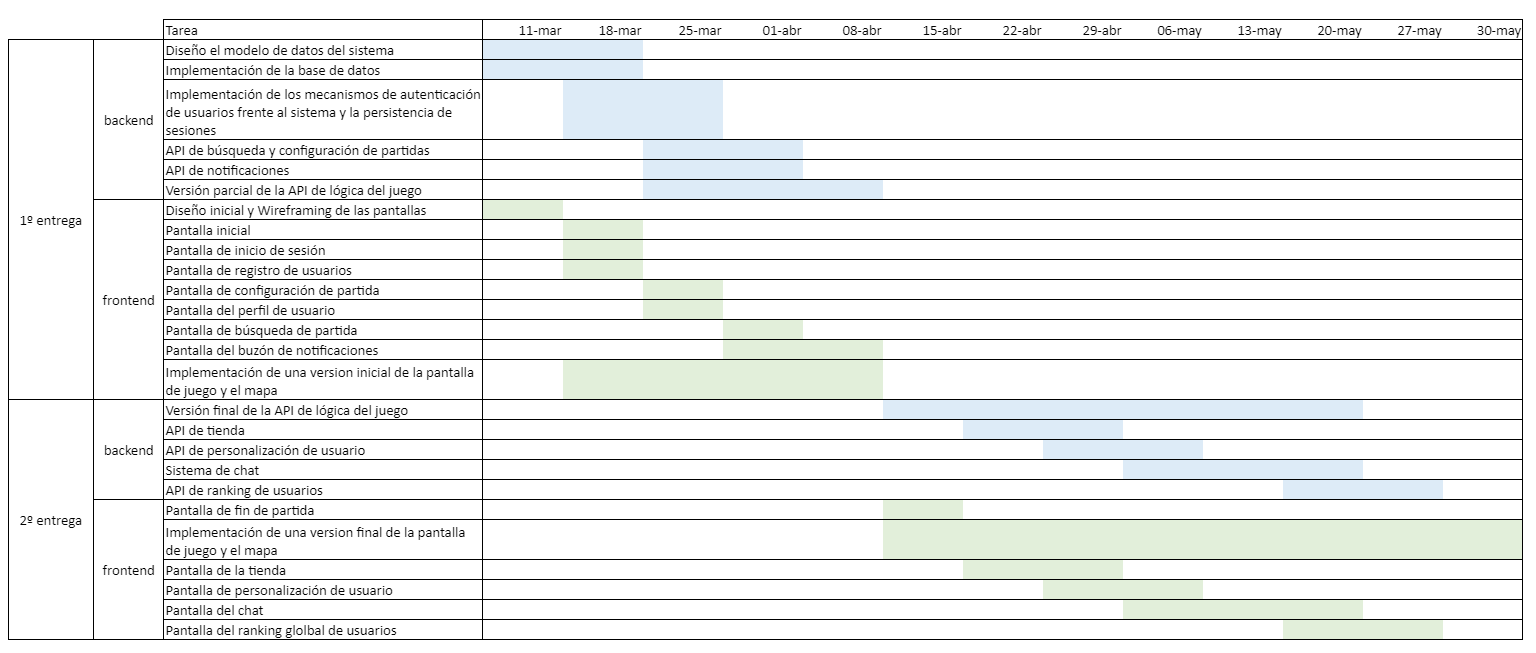
\includegraphics[scale=0.6]{diagramas/gant.PNG}
    \caption{Diagrama de Gantt.}
    \label{fig:my_label}
\end{figure}
\end{landscape}

Se han establecido las siguiente divisiones de trabajo junto a las personas asignadas a cada parte:

\begin{itemize}
    \item \textbf{Backend}: Guillermo Enguita y Samuel García
    \item \textbf{Frontend}
    \begin{itemize} 
        \item \textbf{Angular}: Laura González y Jorge Grima
        \item \textbf{React}: Fran Crespo y Emilio Estevan
    \end{itemize}
\end{itemize}

La división de tareas diarias internas en cada uno de los equipos se consensuará entre sus miembros, y se preferirá en todo momento la programación por pares.\\

Tanto el \textit{frontend} como el \textit{backend} poseerán un calendario de seguimiento propio en el cual se establecen los objetivos a realizar junto a sus fechas limite para ser completadas. \\

Ambos tienen en común dos fechas las son \textbf{8 de abril} debido a que esta es la es la entrega intermedia, en donde se le mostrará al cliente una primera versión funcional del proyecto
y \textbf{30 de junio} porque esta es la fecha de la entrega del proyecto.\\

Cada dos semanas todos los miembros del equipo rellenarán un cuestionario indicando las horas trabajadas y el progreso realizado. Por otro lado las actas se tomarán por turnos durante las reuniones con el cliente en las fechas indicadas por él mismo.\\

Las métricas de rendimiento del equipo irán marcadas por el estado por cada una de las incidencias y tareas pendientes de cada uno de los repositorios. Si se diese el caso de que algún equipo quedase rezagado respecto al resto o sufriera algún imprevisto, éste deberá comentárselo al coordinador del equipo para que así se pueda tomar una decisión sobre cómo actuar al respecto. 

\subsubsection{Calendario de seguimiento para el frontend}
El calendario interno para el \textit{frontend} va a ser el mismo para ambas implementaciones. La tabla \ref{table:frontend} muestra las tareas a realizar por este equipo. \newline


\renewcommand{\arraystretch}{1.3}
\begin{table}[hbt!]
\begin{adjustbox}{minipage=18cm, center}
\begin{tabularx}{\textwidth}{|c|X|c| }
\hline
Entrega & Tarea & Fecha objetivo\\ \hline
\multirow{9}{*}{Entrega 1} & Diseño inicial y \textit{Wireframing} de las pantallas & 18 marzo \\\cline{2-3}
& Pantalla inicial & 18 marzo\\\cline{2-3}
& Pantalla de registro de usuario & 18 marzo \\\cline{2-3}
& Pantalla de inicio de sesión &  18 marzo \\\cline{2-3}
& Pantalla del perfil de usuario &  25 marzo \\\cline{2-3}
& Pantalla de búsqueda de partida &  25 marzo \\\cline{2-3}
& Pantalla de configuración de partida & 25 marzo \\\cline{2-3}
& Pantalla del buzón de notificaciones del usuario &  8 abril \\\cline{2-3}
& Implementación de una versión inicial de la pantalla del juego y del mapa & 8 abril
\\\hline
\multirow{6}{*}{Entrega 2} & Pantalla de fin de partida & 15 abril \\\cline{2-3}
& Implementación de una versión final de la pantalla del juego y del mapa & 30 mayo\\\cline{2-3}
& Pantalla de la tienda & 29 abril \\\cline{2-3}
& Pantalla de personalización de usuario & 6 mayo\\\cline{2-3}
& Pantalla del \textit{chat} en la partida & 20 mayo \\\cline{2-3}
& Pantalla de la clasificación global de usuarios& 27 mayo \\\cline{2-3}
\hline
\end{tabularx}
\caption{Tabla de seguimiento del \textit{frontend}}
\label{table:frontend}
\end{adjustbox}
\end{table}
%\end{center}
\FloatBarrier    

\newpage

\subsubsection{Calendario de seguimiento para el backend}
 La tabla \ref{table:backend} muestra las tareas de este equipo a realizar. \newline

\renewcommand{\arraystretch}{1.3}
\begin{table}[hbt!]
\begin{adjustbox}{minipage=18cm, center}
\begin{tabularx}{\textwidth}{|c|X|c| }
\hline
Entrega & Tarea & Fecha objetivo \\\hline
\multirow{6}{*}{Entrega 1}& Diseño el modelo de datos del sistema & 18 marzo\\\cline{2-3}
 & Implementación de la base de datos & 18 marzo \\\cline{2-3}
 & Implementación de los mecanismos de autenticación de usuarios frente al sistema y la persistencia de sesiones & 25 marzo \\\cline{2-3}
 & \textit{API} de búsqueda y configuración de partidas & 25 marzo\\\cline{2-3}
 & \textit{API} de notificaciones &  1 abril \\\cline{2-3}
 & Versión parcial de la \textit{API} de lógica del juego & 8 abril \\\cline{2-3}
\hline
\multirow{5}{*}{Entrega 2} & Versión final de la \textit{API} de lógica del juego & 20 mayo \\\cline{2-3}
& \textit{API} de la tienda & 29 abril \\\cline{2-3}
& \textit{API} de personalización de usuario& 6 mayo \\\cline{2-3}
& Sistema de \textit{chat} & 20 mayo \\\cline{2-3}
& \textit{API} de la clasificación de usuarios &  27 mayo \\\cline{2-3}
\hline
\end{tabularx}
\caption{Tabla de seguimiento del \textit{backend}}
\label{table:backend}
\end{adjustbox}
\end{table}
\FloatBarrier
 
La responsable del seguimiento de todos estos aspectos será Laura González.

\section{Análisis y diseño del sistema}

\subsection{Análisis de requisitos}
Los requisitos funcionales de nuestra aplicación se pueden encontrar detallados en la tabla \ref{tab:rf}. La tabla \ref{tab:rnf} recoge los requisitos no funcionales. Ambos tipos de requisitos se encuentran claramente detallados e identificados, para facilitar su referencia en documentación futura.
\renewcommand{\arraystretch}{1.3}
\begin{table}[h!]
    \centering
    \begin{tabularx}{\textwidth}{|l|X|}
    \hline
         Código & Descripción  \\
         \hline
         RF-1 & El sistema permitirá a los usuarios registrarse, utilizando un correo electrónico y estableciendo un nombre de usuario y una contraseña.\\
         \hline
         RF-2 & El sistema permitirá a los usuarios iniciar sesión, utilizando su correo electrónico y su contraseña.\\
         \hline
         RF-3 & El sistema permitirá a los usuarios iniciar sesión, utilizando su nombre de usuario y su contraseña.\\
         \hline
         RF-4 & El sistema proporcionará a los usuarios un juego de \textit{Risk}.\\
         \hline
         RF-5 & El sistema ofrecerá a los usuarios un menú que permitirá buscar partidas públicas en curso, destacando las partidas en las que participen sus amigos.\\
         \hline
         RF-6 & El sistema recompensará a los jugadores al ganar partidas, otorgándoles puntos canjeables.\\
         \hline
         RF-7 & El sistema ofrecerá una tienda a los usuarios en la que podrán utilizar los puntos descritos en el requisito \textbf{RF-6} para comprar diferentes cosméticos que permitan la personalización. \\
         \hline
         RF-8 & El sistema permitirá a los usuarios personalizar elementos del juego.\\
         \hline
         RF-8.1 & El sistema permitirá a los usuarios modificar su foto de perfil y su biografía.\\
         \hline
         RF-8.2 & El sistema permitirá a los usuarios personalizar sus dados y fichas de juego, utilizando los cosméticos comprados en la tienda definida en el requisito \textbf{RF-7}.\\
         \hline
         RF-8.3 & Las personalizaciones realizadas serán visibles por todos los usuarios.\\
         \hline
         RF-9 & El sistema permitirá a los usuarios gestionar una lista de amigos.\\
         \hline
         RF-10 & El sistema permitirá a los usuarios consultar una clasificación global, la cuál mostrará a los mejores jugadores junto con sus respectivas puntuaciones.\\
         \hline
         RF-11 & El sistema permitirá a los usuarios consultar el perfil personal de otros jugadores.\\
         \hline
         RF-12 & El sistema permitirá a los usuarios crear una partida.\\
         \hline
         RF-12.1 & El sistema permitirá crear partidas públicas, a las que cualquier usuario se podrá unir.\\
         \hline
         RF-12.2 & El sistema permitirá crear partidas privadas, de forma que el usuario deberá definir una contraseña para el acceso a dicha partida.\\
         \hline
         RF-12.3 & El sistema permitirá al usuario establecer el número de jugadores de la partida (de 2 a 6 jugadores).\\
         \hline
         RF-13 & Las partidas se desarrollarán de forma asíncrona.\\
         \hline
         RF-13.1 & Cuando llegue el turno del jugador, el sistema le avisará mostrando una notificación en la pantalla si está conectado a la aplicación.\\
         \hline
         RF-13.2 & Si el usuario no está conectado, el sistema enviará el aviso a través de correo electrónico.\\
         \hline
         RF-13.3 & Si el usuario no realiza su jugada dentro de un tiempo determinado, el sistema lo expulsará de la partida.\\
         \hline
         RF-14 & El sistema ofrecerá un \textit{chat} que permitirá a los jugadores de una partida comunicarse entre ellos.\\
         \hline
    \end{tabularx}
    \caption{Requisitos funcionales de la aplicación.}
    \label{tab:rf}
\end{table}

\newpage
\begin{table}[h!]
    \centering
    \begin{tabularx}{\textwidth}{|l|X|}
         \hline
         Código & Descripción \\
         \hline
         RNF-1 & El usuario necesitará acceso a \textit{Internet} para poder utilizar la aplicación.\\
         \hline
         RNF-2 & La interfaz de la aplicación estará disponible en castellano.\\
         \hline
         RNF-3 & Los usuarios deberán registrarse para poder participar en las partidas.\\
         \hline
         RNF-4 & Un mismo usuario no podrá participar en varias partidas de forma simultánea. \\
         \hline
         RNF-5 & El usuario podrá continuar una partida en curso independientemente del dispositivo con el que se conecte y el cliente que utilice.\\
         \hline
         RNF-6 & La interfaz ofrecida estará adaptada a formatos de pantalla horizontales, habituales en los navegadores \textit{web}, y no ofrecerá capacidades adaptativas para su uso en dispositivos móviles.\\
         \hline
    \end{tabularx}
    \caption{Requisitos no funcionales del sistema.}
    \label{tab:rnf}
\end{table}

\newpage

\subsection{Diseño del sistema}

El diseño y planificación de los elementos y lógica de un sistema es fundamental para su desarrollo. En consecuencia, se han desarrollado los correspondientes diagramas arquitecturales que reflejan los componentes de la aplicación, así como la interacción entre ellos. \newline

En primer lugar, se ha modelado el \textbf{diagrama de componentes}, apreciable en la Figura 2, el cual representa los componentes principales en ejecución, sus interfaces y conectores que les permiten interactuar. Concretamente, se puede apreciar los dos componentes cliente, uno para cada tecnología a utilizar, los cuales implementan la lógica de presentación y contienen parte de lógica interna de la aplicación, y se comunican con el servidor mediante la misma interfaz (\textit{API}). En siguiente lugar, se encuentra el servidor \textit{web}, el cual ofrece una interfaz común a los clientes e implementa la lógica de negocio y el acceso a los datos del sistema. Por último, se encuentra el gestor de base de datos, el cual aporta la persistencia necesaria al sistema.

\begin{figure}[h!]
    \centering
    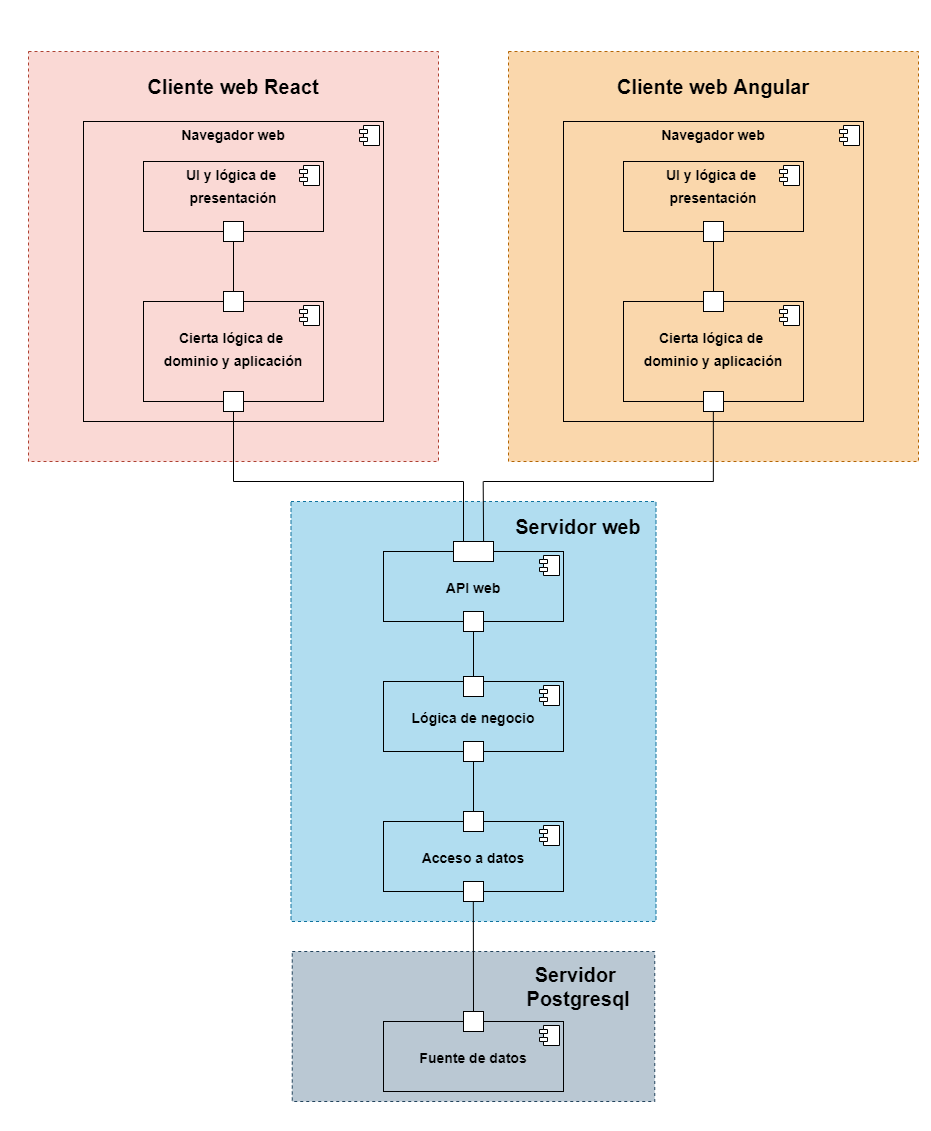
\includegraphics[width=1\linewidth]{diagramas/DC.png}
    \caption{Diagrama de componentes.}
\end{figure}


Por otro lado, en la Figura 3 se ilustra el \textbf{diagrama de despliegue}, donde se puede apreciar la distribución de los distintos nodos que componen el sistema. En consecuencia, se ha representado el servidor \textit{web} junto con los artefactos de comprenden la lógica interna del servidor y el sistema gestor de base de datos. Este nodo da soporte a los dos tipos de clientes posibles, uno con cada tecnología, los cuales implementan cierta lógica interna de la aplicación y se encargan de mostrar y gestionar la interfaz al usuario. 

\begin{figure}[h!]
    \centering
    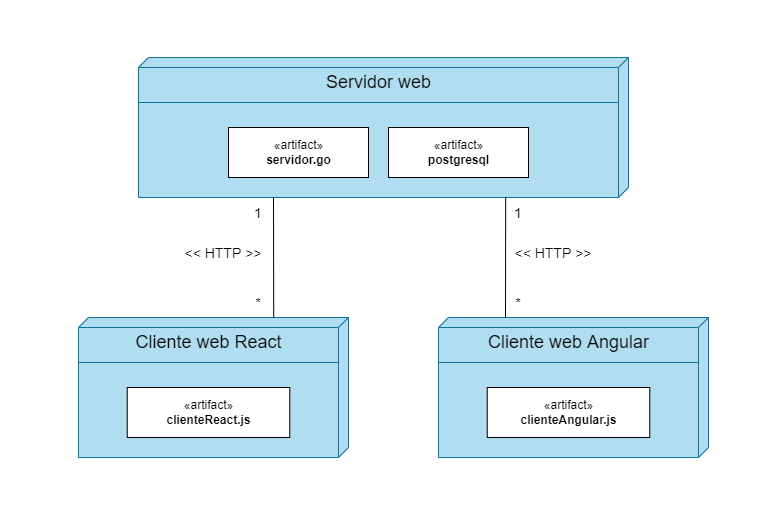
\includegraphics[width=1\linewidth]{diagramas/DD.png}
    \caption{Diagrama de despliegue.}
\end{figure}

Dadas las características del tipo de aplicación \textit{web}, se va a desarrollar una \textbf{arquitectura} cliente-servidor como modelo de diseño, en la que los clientes lanzarán peticiones al servidor, este las gestionará y mantendrá el estado del sistema y su persistencia, y devolverá la respuesta correspondiente. Además, como \textbf{protocolo de comunicación} entre los nodos de la red, se utilizará \textbf{HTTP}.

\subsubsection{Tecnologías elegidas}

En cuanto a las \textbf{tecnologías elegidas}, cabe destacar el uso de \textbf{HTML}, \textbf{CSS} y \textbf{JavaScript} para la parte del frontend de la aplicación, en la que se distinguirá la utilización de dos librerías de creación de interfaces de usuario: \textbf{React} y \textbf{Angular}. Por ello, la aplicación divergirá en dos clientes ligeramente distintos para el usuario e internamente construidos de distinta forma, que se comunicarán con el servidor web central, el cual no distinguirá entre tipos de clientes, sino que se limitará a atender peticiones, gestionarlas y devolver la respuesta adecuada. \newline

Por otro lado, la tecnología elegida para el servidor o backend es el lenguaje \textbf{Go}, ya que es uno de los lenguajes más potentes y con más futuro en sistemas distribuidos, el cual ofrece infinidad de herramientas de gestión para un servidor de las características del sistema. Para la persistencia de datos del sistema, se recurrirá al gestor \textbf{PostgreSQL}, ya que cubre con garantías todas las necesidades de la aplicación. \newline


Para el backend se ha valorado utilizar las siguientes librerías auxiliares para servir contenidos \textbf{HTTP}:

\begin{itemize}
    \item \textit{Frameworks de web}: Se ha valorado utilizar frameworks web como \textbf{Echo} o \textbf{Gin}. Sin embargo, se ha considerado que  la documentación era escasa en todos los \textit{frameworks} evaluados, y su uso forzaría a una dependencia en las mismas. 
    
    \item Por otro lado, se ha optado por utilizar una librería auxiliar a la librería estándar de \textbf{HTTP} de \textbf{Go}, \textbf{Chi}, que se caracteriza por ser solamente una ampliación a la librería estándar muy sencilla de utilizar, y que permite establecer diferentes \textit{middleware} programables para diferentes \textit{URLs}, algo que se va a necesitar.
    
    \item Librerías auxiliares de \textbf{SQL}: Se ha evaluado utilizar \textbf{ORMs} como \textbf{Gorm}, pero se ha considerado que el modelo de datos es lo suficientemente sencillo como para utilizar la librería \textbf{SQL} y consultas tradicionales.
\end{itemize}

\subsubsection{Aspectos a considerar}

Entre otros \textbf{aspectos a considerar}, cabe destacar los siguientes. El despliegue e instalación de la aplicación se llevará a cabo mediante contenedores de \textbf{Docker}, preferiblemente en un sistema operativo \textbf{Linux}, dada la facilidad de uso y el rápido despliegue que ofrece. Por otro lado, el modelo de datos a implementar se limita al estándar \textbf{SQL}, es decir, un modelo relacional. El servidor ofrece una \textit{API Web} de tipo \textbf{REST}, de forma que cada petición contenga toda la información necesaria para comprenderla, sin que exista un estado explícito a consensuar entre cliente y servidor. \newline

Por último, se barajaron otras opciones a las comentadas anteriormente:

\begin{itemize}
    \item Utilizar otro lenguaje para el \textit{backend}, como \textbf{Java}. Sin embargo, se decidió que era más apropiado el uso de \textbf{Go}, que es uno de los lenguajes para sistemas distribuidos más usados, ya que ofrece múltiples recursos para soportar distintos protocolos de comunicación, junto con aspectos de seguridad, así como simplicidad, compatibilidad y eficiencia en la gestión de peticiones de red dentro de su propia librería estándar. Además, el equipo está habituado al desarrollo de aplicaciones web con \textbf{Go}, hecho que impulsa su utilización.
    
    \item  Manejar otro sistema gestor de base de datos similar, como un gestor de bases de datos \textbf{NoSQL}. Actualmente existe un amplio abanico de opciones para elegir y como las necesidades de la aplicación se cubren con prácticamente cualquier gestor, se determinó el uso de  \textbf{PostgreSQL} ya que es uno de los gestores de código abierto más utilizados y que ofrece aspectos muy interesantes. También, el equipo está habituado al uso de este gestor en concreto.
    
    \item Existen muchas librerías para el desarrollo de interfaces \textit{web}. Sin embargo, se decidió utilizar  \textbf{React} y \textbf{Angular} porque ofrecen una gran cantidad de recursos que permiten construir elementos complejos mediante instrucciones muy simples, así como el soporte y documentación que tienen dado su extendido uso en la actualidad.
\end{itemize}


%%%%%%%% Entrega 2 y final
%\section{Memoria del proyecto}
%\subsection{Inicio del proyecto}
%\subsection{Ejecución y control del proyecto}
%\subsection{Cierre del proyecto}
%\section{Conclusiones}


\clearpage
%\section{Anexos}
%\subsection{Glosario}
%\subsection{Actas de todas las reuniones realizadas}

\newpage
\section{Referencias}
\subsection{Bibliografía}
\printbibliography

\end{document}
